\documentclass[12pt]{dalcsthesis}
\usepackage{graphicx}
\graphicspath{ {images/} }
\begin{document}
\mcs 
\title{Bridging Data and Electronic Dance Music}
\author{Jasdev Singh}
\defenceday{9}
\defencemonth{March}
\defenceyear{2014}
\convocation{May}{2014}

\supervisor{Dr. Yanjun Qi}
\reader{Matthew N. Eisler, PhD}

\nolistoftables
\nolistoffigures

\frontmatter

\begin{abstract}
Electronic dance music (EDM) is a relatively new genre with unique features such as a myriad of subgenres and the common notion of playing live events in a festival format. With its rise to mainstream popularity, there are opportunities to explore the social dynamics of EDM by analyzing datasets associated with the genre. In our research, we seek to understand three such public datasets, the DJ Magazine Top 100, Electric Zoo Festival set lists, and SoundCloud comment data, at a deeper level. Some of the techniques employed are time-series analyses, network diagrams, and sentiment analysis, to help draw conclusions about this young, but rapidly growing, genre.
\end{abstract}

\begin{acknowledgements}
\begin{itemize}
	\item Dr. Yanjun Qi, PhD
	\item Matthew N. Eisler, PhD
	\item UVa's Association of Computing Machinery
\end{itemize}
\end{acknowledgements}

\mainmatter

\chapter{Introduction}

\section{Background}

Electronic dance music (often called EDM) includes multiple electronic music genres, usually for dance-based events. (typically at festivals or clubs). At these live events, it is very common for DJs to play continuous sets, ranging from 30 minute to multiple hour mixes. Moreover, producers and dee jays (DJs) will often collaborate on and play each other's music. Below is a graph from a recent report by Google Music's Research Group (add citation) showing the popularity of various genres uploaded to the Google Play store (add link), since the service's inception. Highlighted by the red box, it can be seen that EDM is roughly the 6th largest genre as of the most recent year in the survey.

\begin{figure}[h]
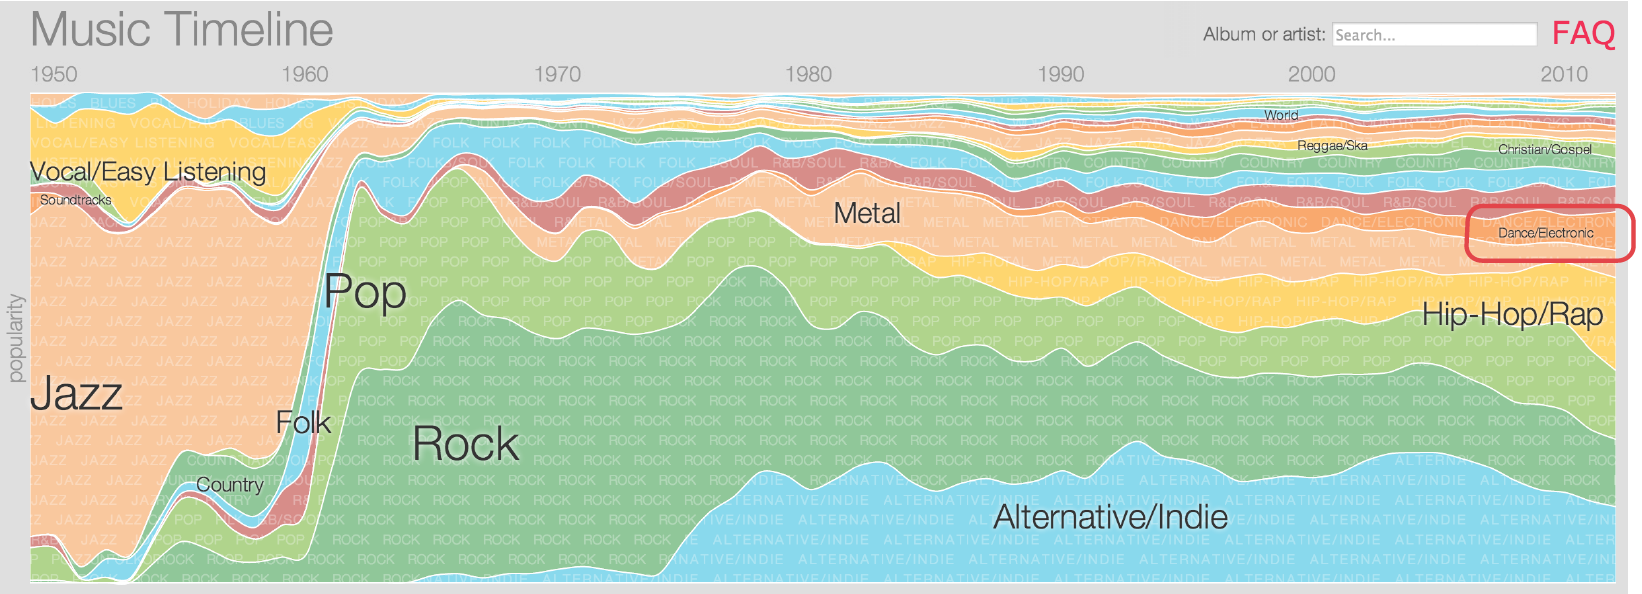
\includegraphics[scale=.49]{genre_graph}
\centering
\end{figure}

\chapter{Motivation}

\section{Previous Work}

\section{Framework}

\chapter{Conclusion}

\bibliographystyle{plain}
\bibliography{simple}

\end{document}
